%%%%%%%%%%%%%%%%%%%%%%%%%%%%%%%%%%%%%%%%%%%%%%%%%%%%%%%%%%%%%%%%%%%%%%%%%%%%%%%
\chapter{Atrito}              % Sem "Experiência 01" ou qualquer outro número
\label{Chap:ExpAtrito}        % para poder trocar a ordem com facilidade
%%%%%%%%%%%%%%%%%%%%%%%%%%%%%%%%%%%%%%%%%%%%%%%%%%%%%%%%%%%%%%%%%%%%%%%%%%%%%%%

\begin{fullwidth}\it
	Realizaremos dois experimentos com o intuito de determinar os coeficientes de atrito estático e cinético entre algumas superfícies. Para a determinação do coeficiente de atrito estático, usaremos um plano com inclinação variável e determinaremos o ângulo de iminência de movimento. Já para a determinação do coeficiente de atrito cinético, verificaremos a aceleração de um bloco quando sujeito a uma tensão constante e a uma força de atrito que atua no sentido de retardar o movimento, permitindo que o coeficiente de atrito cinético seja determinado através das Leis de Newton. Utilizaremos os conceitos de medidas, algarismos significativos, gráficos, e regressão quadrática.
\end{fullwidth}

%%%%%%%%%%%%%%%%%%%%%%%%%%%%%%
\section{Regressão quadrática}
%%%%%%%%%%%%%%%%%%%%%%%%%%%%%%

Sempre que acreditamos que os dados experimentais seguem uma tendência linear, podemos utilizar uma regressão linear para determinar a reta que melhor descreve os dados. Em algumas situações, mesmo que os dados não tenham uma tendência linear, podemos obter uma tendência linear ao realizarmos uma mudança de variável. Em algumas situações, no entanto, nenhuma desses dois cenários é viável. Nesses casos, devemos procurar outras formas funcionais para descrever os dados, sendo que para cada forma deve ser possível ajustar uma ``melhor curva''.

Para o caso especial de polinômios de grau dois, isto é, para curvas com a forma
\begin{equation}
    y = A + B x + C x^2,
\end{equation}
%
os coeficientes podem ser calculados através de
\begin{equation}
\begin{pmatrix}
\sum x_i^4 & \sum x_i^3 & \sum x_i^2 \\ \sum x_i^3 & \sum x_i^2 & \sum x_i \\ \sum_i^2 & \sum x_i & n \end{pmatrix} \begin{pmatrix} C \\ B \\ A \end{pmatrix} = \begin{pmatrix} \sum x_i^2y_i \\ \sum x_iy_i \\ \sum y_i \end{pmatrix},
\end{equation}
%
sendo que tal equação tem que ser resolvida para determinar o vetor $\vec{x} = (C, B, A)$. O coeficiente $r^2$ agora se torna uma medida da correlação quadrática, porém sua interpretação segue a mesma, sendo calculado através de
\begin{equation}
    r^2 = 1 - \frac{\sum (y_i - C x_i^2 - B x_i - A)^2}{\sum (y_i - \mean{y})^2}.
\end{equation}
%
O cálculo dos coeficientes $A$, $B$, $C$, e $r^2$ através das equações acima é muito trabalhoso para ser feito manualmente, porém é algo relativamente simples de se implementar em um computador ou mesmo em uma calculadora. A maioria das calculadoras científicas e softwares com algum suporte a tratamento estatístico de dados disponibiliza métodos simples para determinar tais valores de maneira rápida.

%%%%%%%%%%%%%%%%%%%%%%%%%%%%%%%%%%%%%%%%%%%%%%%%%%%%%%%%%%%%%%%%%%%%%%%%%%%%%%%
\section{Força de atrito}
%%%%%%%%%%%%%%%%%%%%%%%%%%%%%%%%%%%%%%%%%%%%%%%%%%%%%%%%%%%%%%%%%%%%%%%%%%%%%%%

%%%%%%%%%%%%%%%%%%%%%%%%%%%%%%%%%%%%%%%%%%%%%%%%%%%%%%%%%%%%%%%%%%%%%%
\subsection{Determinação do coeficiente de atrito estático}
%%%%%%%%%%%%%%%%%%%%%%%%%%%%%%%%%%%%%%%%%%%%%%%%%%%%%%%%%%%%%%%%%%%%%%

\begin{marginfigure}[5cm]
\centering
\begin{tikzpicture}[>=Stealth, rotate=-35,
     interface/.style={
        % superfície
        postaction={draw,decorate,decoration={border,angle=-45,
                    amplitude=0.2cm,segment length=2mm}}},
    ]
      
    \draw[interface] (0,0) -- (4,0);
    \draw[pattern= dots] (1.5,0) rectangle (2.5,1);
        
    \draw[fill] (2,0.5) circle (1pt);
    \draw[->, thick] (2,0.5) -- +(-55:1) node[left]{$\vec{P}$};
    \draw[->, thick] (2,1) -- +(0,0.81915) node[below right]{$\vec{N}$};
    \draw[->, thick] (1.5,0) -- +(-0.573576,0) node[above]{$\vec{f}_{at}$};
    
    \node at (3,1) {$\vec{a} = 0$};
    
    \draw[dashed] (4,0) -- +(-145:1) coordinate (A);
    
    \coordinate (B) at (4,0);
    \coordinate (C) at (0,0);
    
    \pic [draw, "$\theta$", angle eccentricity=1.5] {angle = C--B--A};

\end{tikzpicture}
\caption{Bloco em equilíbrio devido à força de atrito sobre um plano inclinado.}
\end{marginfigure}

Uma maneira simples de determinar o coeficiente de atrito estático entre dois tipos de superfícies consiste em utilizar um plano cuja inclinação pode ser alterada, sobre o qual apoiamos um bloco. Quando o plano for inclinado até que o bloco esteja na iminência de se mover, podemos analisar o sistema ainda como uma situação de equilíbrio.

\begin{marginfigure}
\centering
\begin{tikzpicture}[>=Stealth, rotate=-35,
     interface/.style={
        % superfície
        postaction={draw,decorate,decoration={border,angle=-45,
                    amplitude=0.2cm,segment length=2mm}}},
    ]
      
    \draw[interface, gray] (0,0) -- (4,0);
    \draw[pattern= dots, draw = gray, pattern color = gray] (1.5,0) rectangle (2.5,1);
        
    \draw[fill, gray] (2,0.5) coordinate (center) circle (1pt);
    \draw[->, thick] (2,0.5) -- +(-55:1) node[left]{$\vec{P}$} coordinate (P);
    \draw[->, thick] (2,1) -- +(0,0.81915) node[below right]{$\vec{N}$};
    \draw[->, thick] (1.5,0) -- +(-0.573576,0) node[above]{$\vec{f}_{at}$};
    
    \node at (3,1) {$\vec{a} = 0$};
    
    \draw[dashed] (4,0) -- +(-145:1) coordinate (A);
    
    \coordinate (B) at (4,0);
    \coordinate (C) at (0,0);
    
    \pic [draw, "$\theta$", angle eccentricity=1.5] {angle = C--B--A};
    
    \draw[dashed, ->] (0.5,0.5) -- (3.5,0.5) node[below left]{$x$};
    \draw[dashed, ->] (2,-1) coordinate (X) -- (2,2.5) node[left]{$y$};
    
\end{tikzpicture}
\caption{Sistema de referência para a análise do sistema.\label{Fig:DetCoefAtEstatico}}
\end{marginfigure}

Uma escolha razoável para o eixo $x$ é adotá-lo como paralelo ao plano inclinado (Veja a Figura~\ref{Fig:DetCoefAtEstatico}). Dessa forma o ângulo entre a força peso e o eixo $y$ será o mesmo que aquele entre o plano inclinado e a horizontal. As demais forças estarão em um eixo somente. Aplicando a Segunda Lei de Newton aos eixos, temos:
\begin{description}
    \item[Eixo $x$:] Neste eixo temos, sabendo que $a_x = 0$,
        \begin{align}
            F_{R, x} &= m a_x \\
            P_x + f_{\text{at, x}} + N_x &= 0 \\
            P \sen\theta - \mu_e N &= 0 \\
            mg \sen\theta - \mu_e N &= 0 \\
            mg \sen\theta &= \mu_e N \label{coef_atrito_deduc}
        \end{align}
    \item[Eixo $y$:] Novamente, a aceleração é nula, o que nos leva a
        \begin{align}
            F_{R, y} &= m a_y \\
            N_y + P_y + f_{\text{at, y}} &= 0 \\
            N &= P\cos\theta \\
            N &= mg \cos\theta
        \end{align}
\end{description}
%
Utilizamos acima o fato de que o ângulo entre o peso e o eixo $y$ é igual ao ângulo $\theta$ entre a superfície do plano inclinado e a horizontal.

Substituindo a expressão acima para a força normal na Equação~\eqref{coef_atrito_deduc}, obtemos
\begin{equation}
    \mu_e mg \cos\theta = mg \sen\theta,
\end{equation}
%
o que resulta em
\begin{equation}\label{Eq:CoefAtritoEstaticoMaxTanTheta}
    \mu_e = \tan\theta.
\end{equation}
%
Experimentalmente, basta elevar lentamente a inclinação do plano até que o bloco comece a deslisar. Registrando o ângulo para o qual o movimento inicia, temos um valor limite para o ângulo. Repetindo o procedimento algumas vezes, podemos determinar com alguma precisão qual é o ângulo para o qual temos iminência de movimento.

%%%%%%%%%%%%%%%%%%%%%%%%%%%%%%%%%%%%%%%%%%%%%%%%%%%%%%%%%%%
\subsection{Determinação do coeficiente de atrito cinético}
\label{Sec:AtritoCinetico}
%%%%%%%%%%%%%%%%%%%%%%%%%%%%%%%%%%%%%%%%%%%%%%%%%%%%%%%%%%%

De um ponto de vista prático, o coeficiente de atrito cinético pode ser determinado através de uma análise em que medimos a aceleração a que um corpo sujeito à força de atrito cinético está sujeito. Se, por exemplo, tomarmos a Figura~\ref{Fig:BlocoSujeitoATensaoEAtrito}, na qual um bloco repousa sobre uma superfície horizontal e passa a ser puxado por uma tensão constante $\vec{T}$, estando também sujeito a uma força de atrito cinético $\vec{f}_{at}$, observaremos que ele sofre uma aceleração. Certamente tal aceleração será menor do que no caso em que não existe atrito, sendo que seu valor dependerá diretamente do coeficiente de atrito cinético $\mu_c$ entre a superfície de apoio e a superfície inferior do bloco.

\begin{marginfigure}
\begin{tikzpicture}[>=Stealth,
     interface/.style={
        % superfície
        postaction={draw,decorate,decoration={border,angle=-45,
                    amplitude=0.2cm,segment length=2mm}}},
    ]

	% mesa
	\draw[interface, gray] (-0.25,0) -- (3,0);
	\draw[interface, gray] (3,0) -- (3,-1);
	
	% roldana	
	\draw (3.3,0.05) circle[radius = 0.2];
	\draw[fill] (3.3,0.05) circle[radius = 0.05];
	\draw[fill] (2.6,0.1) rectangle (3.3,0);
	\draw[fill] (2.7,0.1) circle[radius = 0.05];
	\draw[fill] (2.9,0.1) circle[radius = 0.05];
	\draw[fill, white] (3.3,0.05) circle[radius = 0.02];
	
	% bloco superior
	\node[draw, densely dotted, circle, scale = 0.8] (b1) at (0.3,0.7) {1};
	\draw[pattern = north west lines, pattern color = gray, draw = gray] (0.5,0) rectangle +(1,0.5);
	\draw (1.5,0.25) -- (3.3,0.25);
	\draw[->, thick] (1,0.25) -- +(0,-1) node[left]{$\vec{P}_1$};
	\fill (1,0.25) circle (1.5pt);
	\draw[->, thick] (1.5,0.25) -- +(0.5,0) node[above]{$\vec{T}$};
	\draw[->, thick] (1,0.5) -- +(0,1) node[left]{$\vec{N}$};
	\draw[->, thick] (0.5,0) -- +(-0.5,0) node[below right]{$\vec{f}_{at}$};
	
	% bloco inferior
	\node[draw, densely dotted, circle, scale = 0.8] (b2) at (3.1,-1.9) {2};
	\draw (3.5,0.05) -- +(0,-1);
	\draw[pattern = north west lines] (3.3,-0.95) rectangle +(0.4,-0.8);
	\draw[->, thick] (3.5,-0.95) -- +(0,0.5) node[right]{$\vec{T}$};
	\draw[->, thick] (3.5,-1.35) -- +(0,-0.75) node[right]{$\vec{P}_2$};
	\fill (3.5,-1.35) circle (1.5pt);
	
	% Coordenadas
	\draw[->, dashed] (0,0.25) -- (2.5,0.25) node[above]{$x_1$};
	\draw[->, dashed] (1,-1.5) -- (1,2) node[below right]{$y_1$};
	
	\draw[<-, dashed] (3.5, -1.35) +(0,2.25) node[below right]{$y_2$} -- +(0,-1.5);
	\draw[->, dashed] (3.5,-1.35)+(-1,0) -- +(1,0) node[below left]{$x_2$};
	
	\draw[->] (1, 2.5) -- node[above]{$\vec{d}$} +(1,0);
\end{tikzpicture}
\caption{Bloco sujeito à força de atrito cinético durante um deslocamento.\label{Fig:BlocoSujeitoATensaoEAtrito}}
\end{marginfigure}

Podemos determinar uma relação entre $a$ e $\mu_c$ ao aplicarmos a Segunda Lei de Newton ao sistema:
\begin{description}
    \item[Bloco 1:] Aplicando a Segunda Lei de Newton para cada eixo:
        \begin{description}
            \item[Eixo $x_1$:]
                \begin{align}
                    F_{R, x_1} &= m_1 a_{1,x_1} \\
                    T_x + N_x + P_{1,x} + f_{at,x} &= m_1 a_{1,x_1} \\
                    T - f_{at} &= m_1 a_{1,x_1}. \label{Eq:AtritoAtwoodHorizX1}
                \end{align}
            \item[Eixo $y_1$:]
                \begin{align}
                    F_{R, y_1} &= m_1 a_{1,y_1} \\
                    T_y + N_y + P_{1,y} + f_{at,y} &= m_1 a_{1,y_1} \\
                    N_1 - P_1 &= m_1 a_{1,y_1} \\
                    N_1 - P_1 &= 0 \\
                    N_1 &= P_1 \\
                    &= m_1 g
                \end{align}
        \end{description}
    \item[Bloco 2:] Novamente, aplicando a Segunda Lei de Newton para cada eixo:
        \begin{description}
            \item[Eixo $x_2$:] Não há nenhuma força/componente nesse eixo.
            \item[Eixo $y_2$:]
                \begin{align}
                    F_{R, y_2} &= m_2 a_{2,y_2} \\
                    T_y + P_{2,y} &= m_2 a_{2,y_2} \\
                    T - P_2 &= m_2 a_{2,y_2}. \label{Eq:AtritoAtwoodHorizY2}
                \end{align}
        \end{description}
\end{description}

Para determinar uma relação entre a aceleração e o coeficiente de atrito cinético, precisamos resolver o sistema de equações formado pelas expressões \eqref{Eq:AtritoAtwoodHorizX1} e \eqref{Eq:AtritoAtwoodHorizY2}. No entanto, temos três incógnitas: $a_{1,x}$, $a_{2,y}$ e $T$. Para que possamos resolver este sistema, precisamos de mais uma equação: a relação entre as acelerações dos dois blocos. Se considerarmos que a corda que liga os blocos é inextensível, temos que
\begin{equation}
a_{1,x} = - a_{2,y}.
\end{equation}
%
Assim, se adotarmos $a_{x, 1} \equiv a$, podemos reescrever o sistema como
\begin{equation}
\begin{system}
T - f_{at} & = m_1 a \\
T - P_2 &= -m_2 a,
\end{system}
\end{equation}
%
o que resulta, a partir da soma da primeira equação com o negativo da segunda equação, em
\begin{align}
    T - \mu_c N_1 - T + P_2 &= m_1 a + m_2 a \\
    m_2 g - \mu_c m_1 g &= (m_1 + m_2) a,
\end{align}
%
onde usamos
\begin{equation}
    f_{at} = \mu_c N.
\end{equation}
%
Finalmente, isolando $\mu_c$ obtemos
\begin{equation}\label{Eq:CoefAtritoCineticoAtravesDaAceleracao}
    \mu_c = \frac{m_2}{m_1} - \frac{m_1 + m_2}{m_1} \cdot\frac{a}{g}.
\end{equation}

Para que possamos determinar o valor do coeficiente de atrito, basta determinarmos a aceleração através da cinemática, além de determinar os valores de massa do bloco que repousa sobre a superfície horizontal e do corpo suspenso. De acordo com as equações cinemáticas para movimentos com aceleração constante, podemos escrever
\begin{equation}
    x_f = x_i + v_i t + \frac{a}{2} t^2.
\end{equation}
%
Se coletarmos dados para o tempo necessário para o bloco se deslocar entre uma posição fixa $x_i$ e uma posição $x_f$ cujo valor podemos variar, podemos determinar o valor da aceleração através de uma regressão quadrática, por meio do coeficiente $C$. É claro que se pudermos garantir que a velocidade inicial $v_i$ é nula, então é possível utilizar uma mudança de variável $\tau = t^2$ e empregar uma regressão linear para determinar a aceleração. Na prática, no entanto, é muito difícil eliminar a velocidade inicial. Nesse caso, a regressão quadrática resulta em valores muito mais precisos para a aceleração do sistema.

%%%%%%%%%%%%%%%%%%%%%%%%%%%%%%%%%%%%%%%%%%%%%%%%%%%%%%%%%%%%%%%%%%%%%%%%%%%%%%%
\section{Experimento}
%%%%%%%%%%%%%%%%%%%%%%%%%%%%%%%%%%%%%%%%%%%%%%%%%%%%%%%%%%%%%%%%%%%%%%%%%%%%%%%

Inicialmente, vamos utilizar um plano com inclinação variável para determinar o coeficiente de atrito estático entre um bloco e uma superfície. Aumentaremos o ângulo de inclinação progressivamente, até que o bloco passe a deslizar. Considerando tal ângulo como uma aproximação para o ângulo de iminência de movimento, determinaremos o coeficiente de atrito estático através da Equação~\eqref{Eq:CoefAtritoEstaticoMaxTanTheta}.

\begin{figure}[htb]\forcerectofloat
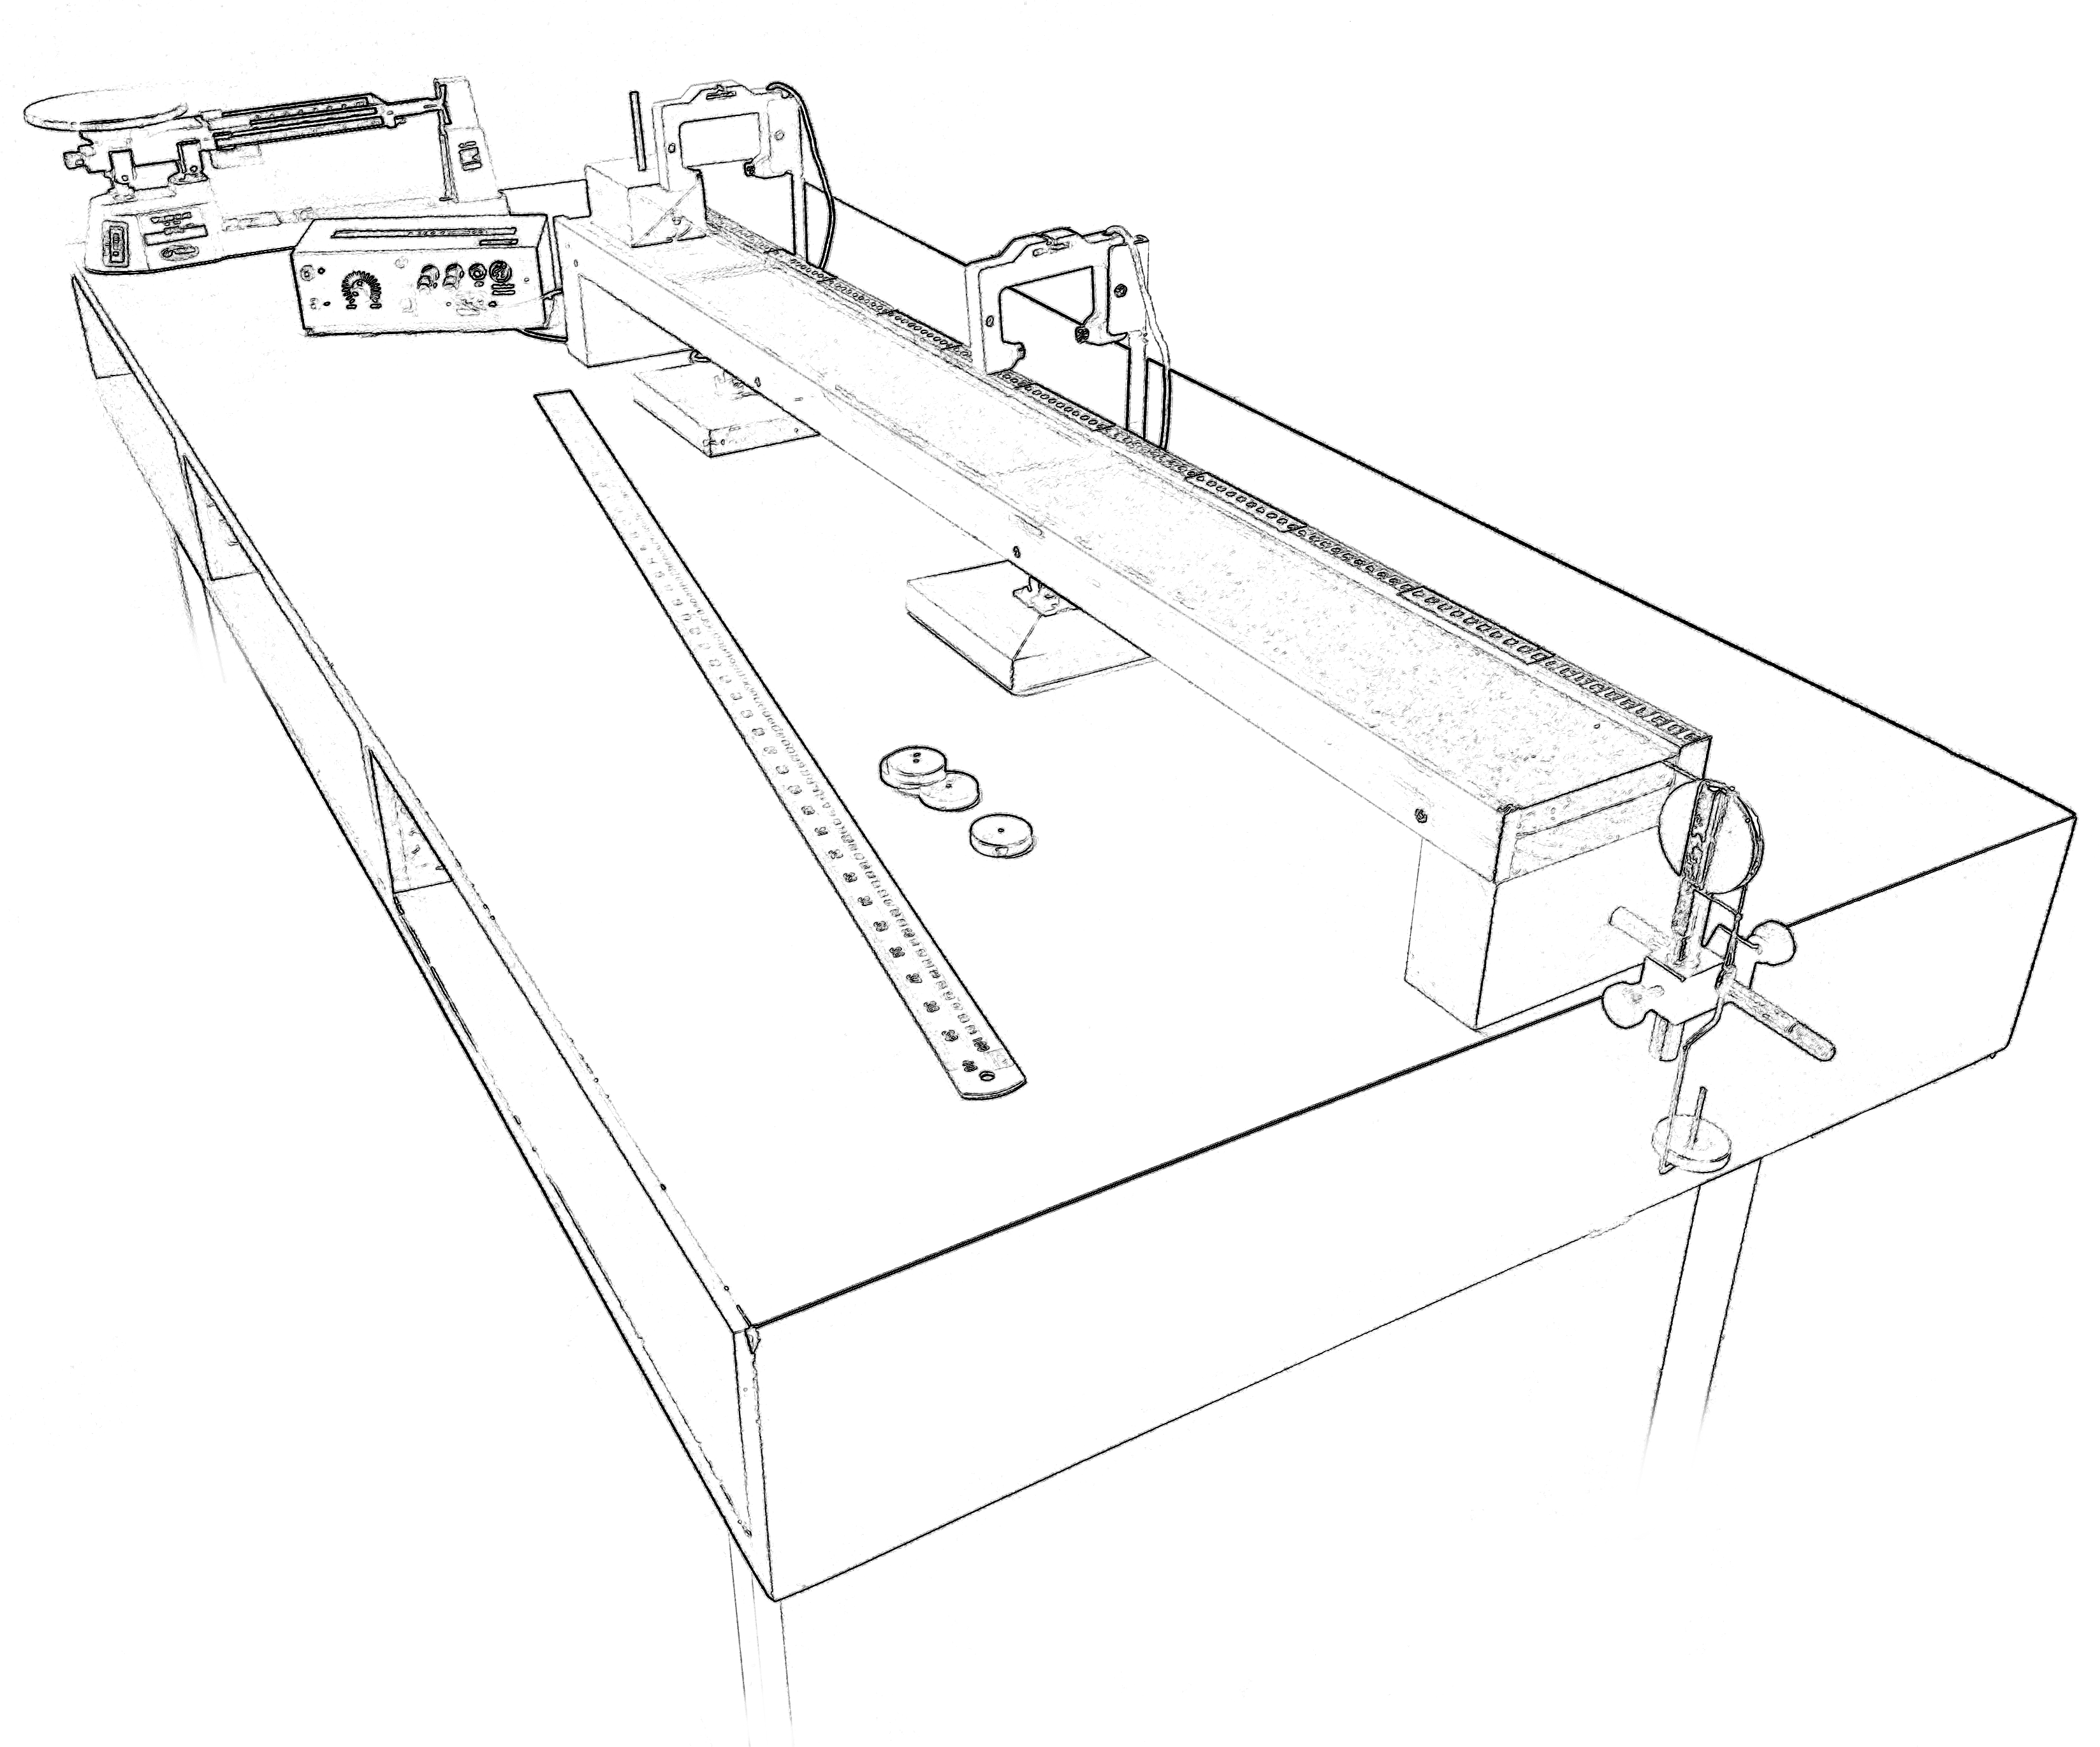
\includegraphics[width=10cm]{Ilustrations/AparatoAtritoCinetico.png}
\caption{Aparato para a determinação do coeficiente de atrito cinético.\label{Fig:AparatoAtritoCinetico}}
\end{figure}

Em um segundo momento, vamos utilizar o aparato mostrado na Figura~\ref{Fig:AparatoAtritoCinetico}, cuja descrição esquemática é dada pela Figura~\ref{Fig:BlocoSujeitoATensaoEAtrito} e cujas propriedades dinâmicas são descritas na Seção~\ref{Sec:AtritoCinetico}, para determinar o coeficiente de atrito cinético. Vamos coletar dados de deslocamento do bloco apoiado sobre a superfície horizontal de forma que possamos determinar a aceleração do sistema utilizando as equações da cinemática. Através do valor dessa variável, poderemos determinar o coeficiente de atrito cinético através da Equação~\eqref{Eq:CoefAtritoCineticoAtravesDaAceleracao}.

\pagebreak
%%%%%%%%%%%%%%%%%%%%%%
\subsection{Objetivos}
%%%%%%%%%%%%%%%%%%%%%%

\begin{itemize}
	\item Determinar o coeficiente de atrito estático entre diversos pares de superfícies;
	\item Verificar uma relação quadrática (parabólica) da posição do bloco sujeito à força de atrito cinético, caracterizando o movimento como um MRUV;
	\item Determinar o coeficiente de atrito cinético entre dois pares de superfícies.
\end{itemize}

%%%%%%%%%%%%%%%%%%%%%%%%%%%%%%%%%%%%%%%%%%%%%%%%%%%%%%%%%%%%%%%%%%%%%%%%%%%%%%%
\section{Material Necessário}
%%%%%%%%%%%%%%%%%%%%%%%%%%%%%%%%%%%%%%%%%%%%%%%%%%%%%%%%%%%%%%%%%%%%%%%%%%%%%%%

\begin{itemize}
	\item Pranchas com superfícies uniformes de diversos tipos;
	\item Blocos com superfícies inferiores de diversos tipos;
	\item Aparato para atrito cinético (suporte, sensores óticos, cronômetro eletrônico, gancho, e roldana);
	\item Anilhas;
	\item Balança;
	\item Régua.
\end{itemize}

%%%%%%%%%%%%%%%%%%%%%%%%%%%%%%%%%%%%%%%%%%%%%%%%%%%%%%%%%%%%%%%%%%%%%%%%%%%%%%%
\section{Procedimento Experimental}
%%%%%%%%%%%%%%%%%%%%%%%%%%%%%%%%%%%%%%%%%%%%%%%%%%%%%%%%%%%%%%%%%%%%%%%%%%%%%%%

%%%%%%%%%%%%%%%%%%%%%%%%%%%%%%%%%%%%%%%%%%%%%%%%%%%%%%%%%%%
\subsection{Determinação do coeficiente de atrito estático}
%%%%%%%%%%%%%%%%%%%%%%%%%%%%%%%%%%%%%%%%%%%%%%%%%%%%%%%%%%%
\begin{enumerate}
	\item Tome um dos blocos e uma da pranchas e disponha o bloco sobre a superfície. Anote o tipo da superfície inferior do bloco e o tipo da superfície superior da prancha na Tabela~\ref{DadosAtritoEstatico};
	\item Verifique o comprimento total $L$ da prancha e o anote na Tabela~\ref{DadosAtritoEstatico};
	
	\begin{marginfigure}
\begin{tikzpicture}[>=Stealth,
     interface/.style={
        % superfície
        postaction={draw,decorate,decoration={border,angle=-45,
                    amplitude=0.2cm,segment length=2mm}}},
    ]
    
    \draw[interface] (-0.5,0) -- (4,0) coordinate (A);
    
    \coordinate (O) at (0,0);
    
    \begin{scope}[rotate = 30]
        \draw[pattern = horizontal lines] (O) rectangle (3.5,0.2);
        \draw[pattern = north east lines] (2.75,0.2) rectangle (3.25,0.7);
        
        \draw[dotted] (0,0.2) -- (0,1) (3.5,0.2) -- (3.5,1);
        \draw[|<->|] (0,1.2) -- node[above]{$L$} (3.5,1.2);
    \end{scope}
    
    \draw[dotted] (3.0311, 1.75) -- (3.5,1.75);
    \draw[|<->|] (3.5, 0) -- node[right]{$h$} (3.5,1.75);
    
    \coordinate (B) at (30:1);
    \pic[draw, "$\theta$", angle eccentricity = 1.3, angle radius = 8mm]{angle = A--O--B};
    
\end{tikzpicture}
\caption{Parâmetros para a determinação do ângulo $\theta$ e do coeficiente de atrito estático $\mu_e$.}
\end{marginfigure}

	\item Incline a prancha lentamente até que o bloco escorregue;\label{Item:LoopAtritoEstaticoInicio}
	\item Meça a altura $h$ da extremidade mais alta da prancha em relação à mesa e anote o valor na Tabela~\ref{DadosAtritoEstatico};\label{Item:LoopAtritoEstaticoFim}
	\item Repita o procedimento dos itens \ref{Item:LoopAtritoEstaticoInicio} e \ref{Item:LoopAtritoEstaticoFim} mais duas vezes e anote os resultados na Tabela~\ref{DadosAtritoEstatico}.
	\item Tome outra prancha, com uma superfície diferente e repita os procedimentos dos itens acima, anotando os resultados na Tabela~\ref{DadosAtritoEstatico}
	\item Tome o outro bloco e proceda da mesma forma que para o primeiro, seguindo os itens acima. Anote os resultados na Tabela~\ref{DadosAtritoEstatico}.
\end{enumerate}

%%%%%%%%%%%%%%%%%%%%%%%%%%%%%%%%%%%%%%%%%%%%%%%%%%%%%%%%%%%
\subsection{Determinação do coeficiente de atrito cinético}
%%%%%%%%%%%%%%%%%%%%%%%%%%%%%%%%%%%%%%%%%%%%%%%%%%%%%%%%%%%
\begin{enumerate}
    \item Tome um dos blocos e uma das pranchas. Anote o tipo da superfície inferior do bloco e o tipo da superfície superior da prancha na Tabela~\ref{DadosAtritoCinetico}
    \item Verifique a massa do bloco utilizando a balança, anotando-a na Tabela~\ref{DadosAtritoCinetico}. Disponha-o sobre a prancha, de forma que sua extremidade esteja alinhada ao início da superfície;
    \item Disponha o primeiro sensor\footnote{Tome cuidado para que a posição de tal sensor não seja alterada durante todo o experimento.} a aproximadamente \np[cm]{5,00} da extremidade do bloco oposta ao início da superfície;
    \item Disponha o segundo sensor a aproximadamente \np[cm]{10,00} do primeiro sensor;
    \item Ligue o bloco ao gancho através do fio, passando pela roldana;
    \item Coloque no gancho o menor número de anilhas capaz de fazer com que o bloco deslize. Afira a massa do conjunto formado pelas anilhas e pelo gancho e anote os valores na Tabela~\ref{DadosAtritoCinetico};
    \item Ligue/zere o cronômetro e volte a colocar o gancho na extremidade da corda, deixando-o suspenso. Alinhe o bloco novamente ao início da superfície e o segure, impedindo que o sistema se mova;\label{Item:LoopAtritoCineticoInicio}
    \item Solte o bloco e verifique o tempo cronometrado para a passagem entre os dois sensores. Anote o valor obtido na Tabela~\ref{DadosAtritoCinetico};
    \item Reinicie o cronômetro e volte a determinar o tempo para a passagem do bloco entre os dois sensores mais duas vezes, tomando o cuidado de alinhar a extremidade do bloco ao início da superfície. Anote os valores de tempo obtidos na Tabela~\ref{DadosAtritoCinetico}.
    \item Desloque a posição do segundo sensor em \np[cm]{10,00} em relação ao valor inicial, afastando-o do primeiro sensor;\label{Item:LoopAtritoCineticoFim}
    \item Repita os itens \ref{Item:LoopAtritoCineticoInicio} a \ref{Item:LoopAtritoCineticoFim} anteriores e anote os valores na Tabela~\ref{DadosAtritoCinetico}.
    \item Continue afastando o segundo sensor de \np[cm]{10,00} em \np[cm]{10,00}, coletando os dados de tempo para o deslocamento entre os sensores. A coleta de dados cessará quando a nova posição do segundo sensor for tal que não permita a passagem do bloco pelo sensor antes que o gancho com as anilhas atinja o chão.\footnote{Precisamos garantir que o movimento é acelerado em toda sua extensão. Se o gancho atingir o chão antes de o bloco passar pelo segundo sensor, teremos uma parte do movimento com velocidade constante.}
\end{enumerate}

%%%%%%%%%%%%%%%%%%%%%%%%%%%%%%%%%%%%%%%%%%%%%%%%%%%%%%%%%%%%%%%%%%%%%%%%%%%%%%%
%%%%%%%%%%%%%%%%%%%%%%%%%%%%%%%%%%%%%%%%%%%%%%%%%%%%%%%%%%%%%%%%%%%%%%%%%%%%%%%
%%%%%%%%%%%%%%%%%%%%%%%%%%%%%%%%%%%%%%%%%%%%%%%%%%%%%%%%%%%%%%%%%%%%%%%%%%%%%%%
%%%%%%%%%%%%%%%%%%%%%%%%%%%%%%%%%%%%%%%%%%%%%%%%%%%%%%%%%%%%%%%%%%%%%%%%%%%%%%%
\cleardoublepage

\noindent{}{\huge\textit{Atrito}}

\vspace{15mm}

\begin{fullwidth}
\noindent{}\makebox[0.6\linewidth]{Turma:\enspace\hrulefill}\makebox[0.4\textwidth]{  Data:\enspace\hrulefill}
\vspace{5mm}

\noindent{}\makebox[0.6\linewidth]{Aluno(a):\enspace\hrulefill}\makebox[0.4\textwidth]{  Matrícula:\enspace\hrulefill}

\noindent{}\makebox[0.6\linewidth]{Aluno(a):\enspace\hrulefill}\makebox[0.4\textwidth]{  Matrícula:\enspace\hrulefill}

\noindent{}\makebox[0.6\linewidth]{Aluno(a):\enspace\hrulefill}\makebox[0.4\textwidth]{  Matrícula:\enspace\hrulefill}

\noindent{}\makebox[0.6\linewidth]{Aluno(a):\enspace\hrulefill}\makebox[0.4\textwidth]{  Matrícula:\enspace\hrulefill}

\noindent{}\makebox[0.6\linewidth]{Aluno(a):\enspace\hrulefill}\makebox[0.4\textwidth]{  Matrícula:\enspace\hrulefill}
\end{fullwidth}

\vspace{5mm}

%%%%%%%%%%%%%%%%%%%%%%%%%%%%%%%%%%%%%%%%%%%%%%%%%%%%%%%%%%%%%%%%%%%%%%%%%%%%%%%
\section{Questionário}
%%%%%%%%%%%%%%%%%%%%%%%%%%%%%%%%%%%%%%%%%%%%%%%%%%%%%%%%%%%%%%%%%%%%%%%%%%%%%%%

\begin{question}[type={exam}]{2}
Preencha as colunas de dados das tabelas com o número adequado de algarismos significativos e unidades.
\end{question}

\begin{question}[type={exam}]{2}
Determine os valores médios do coeficiente de atrito estático para cada par de superfícies.
\end{question}

\begin{question}[type={exam}]{2}
Faça um gráfico $x \times \mean{t}$ para os dados obtidos para o movimento do bloco sujeito ao atrito cinético.
\end{question}

\begin{question}[type={exam}]{4}
\begin{enumerate}[label=\roman*.]
\item Faça uma regressão quadrática dos dados obtidos para o movimento do bloco sujeito ao atrito cinético.
\item Compare a equação
\begin{equation}
    x_f = x_i + v_i t + \frac{a}{2} t^2
\end{equation}
%
com a equação quadrática
\begin{equation}
    y = A + B x + C x^2
\end{equation}
%
e determine o valor da aceleração do bloco e sua velocidade inicial, isto é, sua velocidade ao passar pelo primeiro sensor.

\item Utilize o valor obtido para a aceleração para determinar através da Equação~\ref{Eq:CoefAtritoCineticoAtravesDaAceleracao} o valor do coeficiente de atrito cinético.
\end{enumerate}
\end{question}

\vfill
%%%%%%%%%%%%%%%%%%%%%%%%%%%%%%%%%%%%%%%%%%%%%%%%%%%%%%%%%%%%%%%%%%%%%%%%%%%%%%%
\pagebreak
\section{Tabelas}
%%%%%%%%%%%%%%%%%%%%%%%%%%%%%%%%%%%%%%%%%%%%%%%%%%%%%%%%%%%%%%%%%%%%%%%%%%%%%%%

\begin{table}[!ht]
\centering
\begin{tabular}{lp{28mm}p{28mm}p{28mm}l}
\toprule
    & \textbf{Blocos:} \\
    \cmidrule{2-3}
    & \cellcolor[gray]{0.89} Superfície 1: & \cellcolor[gray]{0.92} \\
    & \cellcolor[gray]{0.95} Superfície 2: & \cellcolor[gray]{0.97} \\
    \cmidrule{2-3}
    \\
    & \textbf{Pranchas:} \\
    \cmidrule{2-3}
    & \cellcolor[gray]{0.89} Superfície 1: & \cellcolor[gray]{0.92} \\
    & \cellcolor[gray]{0.95} Superfície 2: & \cellcolor[gray]{0.97} \\
    \cmidrule{2-3}
    \\
	&\multicolumn{3}{l}{\textbf{Dados Experimentais (bloco 1 + superfície 1):}} \\
	\cmidrule{2-4}
	& $L$ & $h$ & $\theta = \arcsen (h/L)$ & \\
	\cmidrule{2-4}
	& \cellcolor[gray]{0.89} & \cellcolor[gray]{0.92} & \cellcolor[gray]{0.89} \\
	& \cellcolor[gray]{0.95} & \cellcolor[gray]{0.97} & \cellcolor[gray]{0.95} \\
	& \cellcolor[gray]{0.89} & \cellcolor[gray]{0.92} & \cellcolor[gray]{0.89} \\	
	\cmidrule{2-4}
    \\
	&\multicolumn{3}{l}{\textbf{Dados Experimentais (bloco 1 + superfície 2):}} \\
	\cmidrule{2-4}
	& $L$ & $h$ & $\theta = \arcsen (h/L)$ & \\
	\cmidrule{2-4}
	& \cellcolor[gray]{0.89} & \cellcolor[gray]{0.92} & \cellcolor[gray]{0.89} \\
	& \cellcolor[gray]{0.95} & \cellcolor[gray]{0.97} & \cellcolor[gray]{0.95} \\
	& \cellcolor[gray]{0.89} & \cellcolor[gray]{0.92} & \cellcolor[gray]{0.89} \\	
	\cmidrule{2-4}
    \\
	&\multicolumn{3}{l}{\textbf{Dados Experimentais (bloco 2 + superfície 1):}} \\
	\cmidrule{2-4}
	& $L$ & $h$ & $\theta = \arcsen (h/L)$ & \\
	\cmidrule{2-4}
	& \cellcolor[gray]{0.89} & \cellcolor[gray]{0.92} & \cellcolor[gray]{0.89} \\
	& \cellcolor[gray]{0.95} & \cellcolor[gray]{0.97} & \cellcolor[gray]{0.95} \\
	& \cellcolor[gray]{0.89} & \cellcolor[gray]{0.92} & \cellcolor[gray]{0.89} \\	
	\cmidrule{2-4}
    \\
	&\multicolumn{3}{l}{\textbf{Dados Experimentais (bloco 2 + superfície 2):}} \\
	\cmidrule{2-4}
	& $L$ & $h$ & $\theta = \arcsen (h/L)$ & \\
	\cmidrule{2-4}
	& \cellcolor[gray]{0.89} & \cellcolor[gray]{0.92} & \cellcolor[gray]{0.89} \\
	& \cellcolor[gray]{0.95} & \cellcolor[gray]{0.97} & \cellcolor[gray]{0.95} \\
	& \cellcolor[gray]{0.89} & \cellcolor[gray]{0.92} & \cellcolor[gray]{0.89} \\	
	\cmidrule{2-4}

\bottomrule
\end{tabular}
\caption[][5mm]{Dados para a determinação do atrito estático.}
\label{DadosAtritoEstatico}
\end{table}

\pagebreak

\begin{table*}[!ht]
\centering
\begin{tabular}{lp{25mm}p{25mm}p{25mm}p{25mm}p{25mm}l}
\toprule
    & \textbf{Massas} & & & \textbf{Superfícies} \\
    \cmidrule{2-3} \cmidrule{5-6}
    & \cellcolor[gray]{0.89} $m_{\text{bloco}}$ & \cellcolor[gray]{0.92} & & \cellcolor[gray]{0.89} Bloco: & \cellcolor[gray]{0.92} \\
    & \cellcolor[gray]{0.95} $m_{\text{gancho e anilhas}}$ & \cellcolor[gray]{0.97} & & \cellcolor[gray]{0.95} Prancha: & \cellcolor[gray]{0.97} \\
    \cmidrule{2-3} \cmidrule{5-6}
    \\
	&\multicolumn{4}{l}{\textbf{Dados Experimentais}} \\
	\cmidrule{2-6}
	& $x_0$ & $x_f$ & $t_1$ & $t_2$ & $t_3$ & \\
	\cmidrule{2-6}
	& \cellcolor[gray]{0.89} & \cellcolor[gray]{0.92} & \cellcolor[gray]{0.89} & \cellcolor[gray]{0.92} & \cellcolor[gray]{0.89} \\
	& \cellcolor[gray]{0.95} & \cellcolor[gray]{0.97} & \cellcolor[gray]{0.95} & \cellcolor[gray]{0.97} & \cellcolor[gray]{0.95} \\
	& \cellcolor[gray]{0.89} & \cellcolor[gray]{0.92} & \cellcolor[gray]{0.89} & \cellcolor[gray]{0.92} & \cellcolor[gray]{0.89} \\
	& \cellcolor[gray]{0.95} & \cellcolor[gray]{0.97} & \cellcolor[gray]{0.95} & \cellcolor[gray]{0.97} & \cellcolor[gray]{0.95} \\
	& \cellcolor[gray]{0.89} & \cellcolor[gray]{0.92} & \cellcolor[gray]{0.89} & \cellcolor[gray]{0.92} & \cellcolor[gray]{0.89} \\
	& \cellcolor[gray]{0.95} & \cellcolor[gray]{0.97} & \cellcolor[gray]{0.95} & \cellcolor[gray]{0.97} & \cellcolor[gray]{0.95} \\
	& \cellcolor[gray]{0.89} & \cellcolor[gray]{0.92} & \cellcolor[gray]{0.89} & \cellcolor[gray]{0.92} & \cellcolor[gray]{0.89} \\
	& \cellcolor[gray]{0.95} & \cellcolor[gray]{0.97} & \cellcolor[gray]{0.95} & \cellcolor[gray]{0.97} & \cellcolor[gray]{0.95} \\
	& \cellcolor[gray]{0.89} & \cellcolor[gray]{0.92} & \cellcolor[gray]{0.89} & \cellcolor[gray]{0.92} & \cellcolor[gray]{0.89} \\
	& \cellcolor[gray]{0.95} & \cellcolor[gray]{0.97} & \cellcolor[gray]{0.95} & \cellcolor[gray]{0.97} & \cellcolor[gray]{0.95} \\
	\cmidrule{2-6}
\\
	& \multicolumn{3}{l}{\textbf{Dados calculados}} \\
	\cmidrule{2-3}
	& $\Delta x$ & $\mean{t}$ \\
	\cmidrule{2-3}
	& \cellcolor[gray]{0.89} & \cellcolor[gray]{0.92}  \\ 
	& \cellcolor[gray]{0.95} & \cellcolor[gray]{0.97}  \\ 
	& \cellcolor[gray]{0.89} & \cellcolor[gray]{0.92}  \\ 
	& \cellcolor[gray]{0.95} & \cellcolor[gray]{0.97}  \\ 
	& \cellcolor[gray]{0.89} & \cellcolor[gray]{0.92}  \\ 
	& \cellcolor[gray]{0.95} & \cellcolor[gray]{0.97}  \\ 
	& \cellcolor[gray]{0.89} & \cellcolor[gray]{0.92}  \\ 
	& \cellcolor[gray]{0.95} & \cellcolor[gray]{0.97}  \\ 
	& \cellcolor[gray]{0.89} & \cellcolor[gray]{0.92}  \\ 
	& \cellcolor[gray]{0.95} & \cellcolor[gray]{0.97}  \\ 
	\cmidrule{2-3}
\bottomrule
\end{tabular}
\caption[][5mm]{Dados para a determinação do atrito cinético.}
\label{DadosAtritoCinetico}
\end{table*}
